
\chapter{Conclusion --- orthography}
\label{cha:orth-concl}

Part~\ref{part:orthography} demonstrated that the orthography of lenition may be employed to establish the date of composition of \gls{mw} texts. These developments are summarised in Table~\ref{tab:arolwg}. Any \gls{mw} text consistently applying any of the patterns described in this table may be dated to its appropriate period.

\begin{table}[h]
  \centering
  \caption{The orthographical development of lenition.}
  \label{tab:arolwg}
  \begin{tabular}{rcccl}
    \toprule
    \multicolumn{1}{c}{Period} & \tch{\xT} & \tch{\lT} &  \tch{\xD} & \multicolumn{1}{c}{Other \gls{l}\gls{C}} \\
    \midrule
    \gls{ow} & \mw{p, t, c} & \mw{{p, t, c}} & \mw{b, d, g} & {Not represented} \\
    <1275\hphantom{--1325}  & \mw{p, t, c} & \mw{{p, t, c}} & \mw{b, d, g} & Represented, except /d r̥/ \\
    1275--1325  & \mw{p, t, c} & \mw{{p, t,} {g}} & \mw{b, d, g} & Represented, except /d r̥/ \\
    ?? & \mw[]{p, t, c} & \mw[]{b, t, g} & \mw[]{b, d, g}  & Represented, except /d r̥/ \\
    >1325 & \mw{p, t, c} & \mw{{b, d, g}} & \mw{b, d, g} & Represented, except /d r̥/\\
    \gls{mow} & \mow[]{p, t, c}& \mow[]{b, d, g} &\mow[]{b, d, g} & Represented\\
    \bottomrule
  \end{tabular}%
\end{table}

This overview only applies when \gls{mw} texts consistently employ a single orthography of lenition. Such straightforwardness is only found when the date of its original composition is in the same period as its extant manuscript witness. The corpus of Chapter~\ref{cha:indep-comp-mwbr} had  these features and so it gave an impression of the orthographical standard of most of the stages in the \gls{mw} period.  In most \gls{mw} texts, however, such a short gap between the original composition of a text and its extant manuscript witnesses is uncommon. The only phase that is insufficiently documented is the phase in which lenited \mw[]{t} was the only voiceless stop not represented, as it is only found in \mw[]{Buchedd Beuno}, because it is a later copy of such a `pure' original text\footnote{See Section~\ref{sec:sims-williams} for a discussion of \mw[]{Buchedd Beuno}.}.

Most \gls{mw} manuscripts postdate the twelfth century, even when the texts they contain are much older. In such cases, instances of lenition may be represented because of modernising tendencies of later scribes. Chapter~\ref{cha:welsh-laws} showed  that such modernisations are incomplete, \ie the pattern of lenition of the original composition is still visible. Different scribes  modernised the orthography of lenition to different extents, but the extent of modernisation never reached 100\% (Figure~\ref{fig:barchartlaws}). This makes even a minority of unlenited \mw[]{p, t, c} instead of \mw[]{b, d, g} indicate composition before the thirteenth century. A singular instance of orthographic lenition has lower evidential value than a singular instance of lack thereof, because a scribe may have been quite thorough in modernising.

Some manuscript texts are copies of copies, so they may show the traces of more than one stage of modernisation. A possible example of this is law manuscript \gls{sK}, a fifteenth-century manuscript with partial lenition of all voiceless stops. Based on this example alone, we may conclude that its original composition predates the middle of the thirteenth century, yet representation of lenition of \mw[]{c} is comparatively more widespread than \mw[]{p, t}. This may be evidence that an intermediate copy written in the late thirteenth century existed as a base for manuscript \gls{sK}.

Scribes who modernised the orthography of lenition did so inconsistently. The same word may be found lenited and unlenited in the same manuscript, even when both words should be lenited according to our knowledge of \gls{mw}. Similarly, an element known to cause lenition may have orthographical lenition following it inconsistently. Chapter~\ref{cha:stemm-mwbuch-dewi} demonstrated that this randomly added orthographical lenition may be employed to reconstruct the stemmatics of multiple manuscript witnesses of a single text.

Whenever a scribe added lenition randomly, he would create a unique fingerprint of instances of lenition that were and were not orthographically represented. Thus, if we find sufficiently similar patterns of lenition and non-lenition in two or more manuscripts, these manuscripts may share a common intermediate ancestor in which such a fingerprint was formed. The existence of such a shared fingerprint may be differentiated from chance correspondences with statistical tests, but it may also have its roots in a convergent development of  unrelated manuscripts.

\section{Dating shifts in orthography and phonology}
\label{sec:change-lenition-as}

Part~\ref{part:orthography} treated the orthographical change of lenited \mw[]{p, t, c} from \mw[]{p, t, c} to \mw[]{b, d, g}.  Part~\ref{part:phonology-phonetics} demonstrated that this change in orthography reflected a change in phonology at some point, but it is not necessarily the case that the changes occurred at the same time. Orthography typically lags behind phonology, and Modern English orthography shows that several hundred years of phonological development may be obscured by orthography.

Still,  some evidence shows that the change in orthography did not lag behind the change in phonology to a great extent. This evidence comes from the  treatment of lenited \mw[]{g} and the ways that lenition was sometimes consciously not written so that a reader would not misread and have to repair his reading\footnote{See Section~\ref{sec:lenited-mwg}}. The case of lenited \mw[]{g} demonstrates that thirteenth-century scribes chose not to write lenition, rather than simply because they had not invented the means yet. In the face of this, it is not a stretch to assume that writing \lT\ with \mw[]{p, t, c} served a similar purpose in ensuring correct pronunciation as \lT; not \xD. This assumption gives reason to believe that the orthographical shift of \lT\ from \mw[]{p, t, c} to \mw[]{b, d, g} lagged very little --- if at all --- behind the phonological shift of \lT\ to \xD.

Another reason to assume the orthographical development had a concurrent development in phonology is that the shift in orthography is somewhat reminiscent of how phonological innovations spread through lexical diffusion. Table~\ref{tab:lexdiffxw} gives an example of how the sound change /χʷ > w/  occurred at different stages at successive points in time in mid Wales. The columns may also be thought of as representing different geographical locations along the path of change~\autocite{Wil_Lexical05}. The merger of \lT\ with \xD\ can be represented using a similar table, which is illustrated by Table~\ref{tab:stagesltxd}.


\begin{table}[h]
  %% https://tex.stackexchange.com/questions/433930/stepped-table-in-booktabs/
  \centering
  \caption[Lexical diffusion of /χʷ > w/.]{Lexical diffusion of /χʷ > w/, adapted from \textcite{Wil_Lexical05}, based on \textcite[214--16]{Che_time77}. \(t_1, t_2\) et cetera represent successive points in time at a single location.}
  \label{tab:lexdiffxw}%
  \begin{tabular}{wwwwq}
    \toprule
    \tch{\(t_1\)} & \tch{\(t_2\)} & \tch{\(t_3\)} & \tch{\(t_4\)} & \tch{gloss} \\
    \midrule
     χware & \multicolumn{1}{|w}{ware} & ware & ware & play\\\cline{2-2}
     χwanen & χwanen & \multicolumn{1}{|w}{wanen} & wanen & flea\\\cline{3-3}
    χwa:ir & χwa:ir & χwa:ir & \multicolumn{1}{|w}{wa:ir} &sister\\
    \bottomrule
  \end{tabular}%
\end{table}%


\begin{table}[h]
  \centering
  \caption{Discernible intermediate stages of the merger between \lT\ and \xD\ in \gls{mw}.}
  \label{tab:stagesltxd}
  \begin{tabular}{wwwwwq}
    \toprule
    \tch{\(t_1\)} & \tch{\(t_2\)} & \tch{\(t_3\)} & \tch{\(t_4\)}  &\tch{\(t_5\)}  & \tch{gloss} \\
    \midrule
    can, i cyd & \multicolumn{1}{|w}{gan, i gyd} & gan, i gyd & gan, i gyd& gan, i gyd & with, together\\\cline{2-2}
    ei coron & ei coron & \multicolumn{1}{|w}{ei goron} & ei goron& ei goron & his crown \\\cline{3-3}
    ei plu & ei plu & ei plu & \multicolumn{1}{|w}{ei blu}&{ei blu}& his feathers \\\cline{4-4}
    ei tad & ei tad & ei tad & {ei tad}& \multicolumn{1}{|w}{ei dad} & his father \\
    \bottomrule
  \end{tabular}%
\end{table}

The orthographical shift of  \lT\  to \xD\ is comparable to lexical diffusion in that it initially applied to a limited set of words or phonemes and then gradually grew to cover more environments. Lexical diffusion of sound change is a phenomenon observed to exist in spoken language, so if the \gls{mw} written language shows this phenomenon, then it is probable that it also existed in the spoken language of its day. Table~\ref{tab:hgcstable} shows a lexically diffuse development involving voiceless stops: the \acrfull{hgcs}. 

\begin{table}[h]
  \centering
  \caption{Discernible intermediate dialect areas in the \acrshort{hgcs}.}
  \label{tab:hgcstable}%
  \begin{tabular}{IIIIIIIq}
    \toprule
    \tch{\(t_1\)} & \tch{\(t_2\)} & \tch{\(t_3\)} & \tch{\(t_4\)} & \tch{\(t_5\)} & \tch{\(t_6\)} & \tch{\(t_7\)} & \tch{gloss} \\
    \midrule
    ik & \multicolumn{1}{|I}{ich} & ich & ich & ich & ich & ich & I \\\cline{2-2}
    maken & maken & \multicolumn{1}{|I}{machen} & machen & machen & machen & machen & make \\\cline{3-3}
    dorp & dorp & dorp & \multicolumn{1}{|I}{dorf} & dorf & dorf & dorf & village \\\cline{4-4}
    dat & dat & dat & dat & \multicolumn{1}{|I}{das} & das & das & that \\\cline{5-5}
    appel & appel & appel & appel & appel & \multicolumn{1}{|I}{apfel} & apfel & apple \\\cline{6-6}
    pund & pund & pund & pund & pund & pund & \multicolumn{1}{|I}{pfund} & pound \\
    \bottomrule
  \end{tabular}%
\end{table}%


The \gls{hgcs} is a development comparable to the merger between \gls{mw} \lT\ and \xD. The \gls{hgcs} involved the Proto-Germanic voiceless stops /p t k/. It also involved  voiced spirants /β ð ɣ/, but I restrict myself to the voiceless stops here. In word-initial position, medially following a consonant, or when doubled, the voiceless stops developed into their corresponding affricates: High German /pf, ts, kx/. Medially between vowels and word-finally, voiceless stops became voiced fricatives: /f, s, x/~\autocite[56--57]{Wat_History76}.  This shift may obviously be called a single shift, in that we may describe it as a general shift from stops towards their corresponding affricates and fricatives (among others). Yet isoglosses separating High German from Low German (the latter of which did not undergo the \gls{hgcs}) show that intermediate dialects underwent some, but not all of these developments. The impact of the \gls{hgcs} increases gradually to the South, and different consonants are affected to different degrees. Figure~\ref{fig:hgcsmap} and Table~\ref{tab:hgcstable} both give impressions of some intermediate dialects. Not all developments are included, however. The extent of, \eg~/k > kx/ is even more limited to the Southern area~\autocite[56n]{Wat_History76}.

\begin{figure}[h]
  \centering
  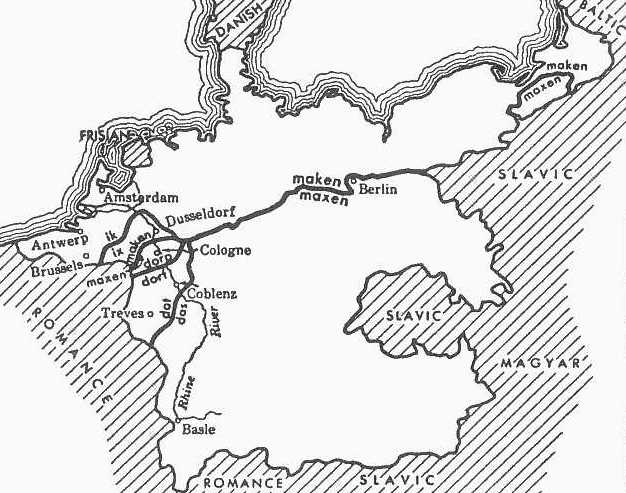
\includegraphics[width=0.8\textwidth]{3orth/images/hgcs.jpg}
  \caption[Bloomfield's isoglosses of the \acrshort{hgcs}.]{The Dutch-German speech area, with the isoglosses of several words containing [k/x], [t/s], and [p/f], from \textcite[344]{Blo_Language33}}
\label{fig:hgcsmap}
\end{figure}

In the \gls{hgcs} we see a single shift of consonants, realised at different levels of completeness in different geographical locations. The merger of \lT\ and \xD\ in \gls{mw} has a temporal rather than a geographical transition zone, and the \gls{hgcs} did not occur overnight either:
\tqt{The spread of the High German shift northward, whatever its ultimate provenience, took place slowly. Although we have demonstrated the occurrence of shifted forms in Alemannic territory for as early as 600, we must not suppose that this change was thoroughgoing and complete at this time. […] Bavarian documents preserve some non-High German forms well into the eighth century and even later. […] And not until the ninth century did the High German consonant shift reach the Middle Franconian dialect.}{Wat_History76}{62}
The fact that the \gls{hgcs} is executed to different levels of completeness along both temporal and geographical axes raises the question as to the initial geographical extent of the merger of \lT\ to \xD\ in \gls{mw}. This matter has remained unsolved in Part~\ref{part:orthography}, but it is obvious that some geographically intermediate stages must have existed for some amount of time.


\section{A review of \gls{mw} lenition rules}
\label{sec:cons-other-ideas}
Knowledge of when orthographical lenition of voiceless stops was introduced in Welsh and knowledge of how scribes changed older texts after this introduction makes it necessary to reconsider what we think we know of \gls{ow} and \gls{mw} grammar. For example, \textcite[2]{schrijver_free_2010}, citing \textcite[18, 179]{evans_grammar_1964} and \textcite[193n]{morgan_y_1952}, states:
`Normally, if a plural subject noun follows the verb, the verb is in the 3sg […]. In early poetry, a plural verb may precede a plural subject, in which case the subject undergoes lenition.' This  archaic rule is illustrated by Examples~\ref{ex:schrsubplv1} and \ref{ex:schrsubplv2}:
\begin{mwl}
  \mwc[ex:schrsubplv1]{CLlH 23.5a}{yn Aber Cuawc yt ganant gogeu}{In Aber Cuawg cuckoos sing}
  \mwc[ex:schrsubplv2]{AP 5.141}{ymgetwynt Gymry}{the Welsh will see to it}
\end{mwl}

The Canu Llywarch Hen poems are thought to have been composed in \gls{ow}, although they survive in \gls{mw} orthography and in fourteenth century manuscripts, and the Book of Taliesin is shown to have added orthographic lenition of \mw[]{c}\footnote{See Section~\ref{sec:haycock}.} Having established that  lenition of voiceless stops was represented in the thirteenth century at the earliest, and having established that fourteenth-century scribes would add orthographical lenition of voiceless stops, we must amend Schrijver's (and Evans' and Morgan's) statement that nominal subjects of plural verbs undergo lenition in early poetry.

Yet Part~\ref{part:orthography} shows that lenition of these consonants was probably added by the fourteenth-century manuscript scribes, rather than the original composers of the poem. It is indeed a feature of early poetry that plural verbs may have nominal subjects, but the lenition following it is not a feature of the early poetry itself, but rather a feature of the fourteenth-century manuscripts.
This means that those seeking to prove that early poetry had lenition of nominal subjects following plural verbs either need to find a lenited nominal subject that has an initial consonant other than \mw[]{p, t, c}, or they must demonstrate that the orthographic lenition of these consonants  precedes the fourteenth century. In fact, \textcite[65--66]{van_development14} does not find subject lenition following plural verbs, but finds instances of non-lenition instead, including one case other than \mw[]{p, t, c} in Example~\ref{ex:vansluissubjlen}:
\mwcc[ex:vansluissubjlen]{RBH 641.38}{A gwrhau a \al{orugant gwyr} y iarllaeth y owein.}{And the noblemen did fealty to Owain’s earldom.}
This example comes from the Red Book of Hergest, dating from around 1400, and the tale itself is much later than the examples given by Schrijver. This curious mix of lenition and non-lenition remains an elusive puzzle, but all the pieces in this puzzle discovered so far belong to the \gls{mw} period, not the \gls{ow} period. Solving this puzzle would improve our knowledge of fourteenth-century Welsh, but it would not directly shed light on the grammar of \gls{ow}\footnote{The examples quoted here curiously show lenition of voiceless stops, and non-lenition of other consonants. If this is indeed the pattern found, then subject lenition following plural verbs may not represent any synchronic stage of Welsh, but may instead show how  fourteenth-century scribes interpreted rules governing lenition in an  the older stage. Then, when updating the orthography of lenition, they would use contemporary orthography for lenition, but non-contemporary rules governing lenition.}.

\section{Outlook}
\label{sec:further-research}
The results presented in Part~\ref{part:orthography} offer avenues for further research. 
Chapter~\ref{cha:stemm-mwbuch-dewi} established that manuscripts sharing lenition or lacking lenition may have a number of agreements beyond what may be attributed to coincidence. Such patterns may be the result of shared inheritance of lenition, \ie a particular lenition fingerprint transmitted into more than one descendant manuscript. Alternatively, however, a similar lenition fingerprint in two or more manuscripts may be the result of a common practice where lenition was added in different degrees in different grammatical environments. To establish a manuscript stemma based on the orthography of lenition, it is necessary to exclude the latter possibility. To exclude this latter possibility whereby shared conventions yield similar patterns of lenition, one must identify the grammatical environments that lenite to different degrees than others. Then, it is possible to calculate whether lenition is modernised independently \emph{within} such a grammatical environment.

The unsolved challenge here is how to categorise types of lenition so that there is no overcategorisation or undercategorisation. If each particle that causes lenition is analysed independently, then sample sizes may be too low to detect a real-world significant correlation between manuscripts. When types of lenition are insufficiently divided, then the possibility remains of similar modernising practices causing similar patterns of lenition. It is, therefore, necessary to understand the specific types of lenition that  are modernised in similar degrees to each another, and differently from other types of lenition. One possible way to do so is to divide between \gls{freelen} and \gls{contlen}; however, it is difficult to identify instances where \gls{freelen} was probably spoken, yet not written, because this type of lenition was in flux. It is, therefore, necessary to find different ways to divide lenition in different classes. One way to do so may be by observing how different types of vowel-consonant or consonant-consonant combinations represent lenition.

Another unsolved issue is the geographical origin of the merger between \lT\ and \xD. In the temporal dimension, we may observe a pattern reminiscent of lexical diffusion with consecutive stages of the merger. In each successive stage, one lenited voiceless stop merges with its radical voiced counterpart and all mergers of previous stages persist. Because such a pattern is frequently observed within the field of dialectology, it is sensible to delve into thirteenth-century Welsh dialectology to see if a geographical as well as a temporal distribution may be found for the merger between \lT\ and \xD.

Yet another avenue for further research is Welsh from before the thirteenth century that survived in later manuscripts. As discussed in Section~\ref{sec:cons-other-ideas}, instances of lenition occurring in these early texts are often additions by later scribes. It would be worthwhile to review which rules governing lenition are believed to be early, yet only survive in comparatively late manuscripts. This analysis may well lead to reconsideration of the lenition rules that belong to each period. Lenition of nominal subjects following a plural verb seems to be an example of such a rule.

Studying the orthography of lenition has some advantages compared to other methods to establish dates for \gls{mw} texts.
One quality is that lenition is ubiquitous in  \gls{mw}; indeed, it is impossible to write any length of text without lenition, which makes the method developed in this thesis applicable to a \gls{mw} text of any length. Compare  this feature with the earlier efforts to use linguistic criteria to date and localise our sources of \gls{mw} discussed in Section~\ref{sec:other-dating-crit}. Consider how \textcite{rodway_dating_2013}, for example, uses the relative frequency of verbal endings to establish dates of texts. One may  effectively employ verbal endings to establish dates, but this method is limited to the appropriate genre or a large corpus. For instance, one may generally date a text using the prevalence of early present subjunctive ending \mw[]{\mbox{-wy}} compared to later \mw[]{\mbox{-o}}, but one may not do so when there are no present subjunctive forms in the first place. A text without subjunctives is conceivable, but a text without lenition is not. The ubiquity of lenition makes it all the more worthwhile to study further the precise date and place that gave the orthography of \lT\ that we know today.

Another remarkable feature of the orthographical development of lenition is the way old orthographical strata may persist even when copied by the most thoroughly modernising scribes. It would be easy for a scribe to write all the instances of \mw[]{\mbox{-wy}} in his exemplar  with \mw[]{\mbox{-o}} in his own manuscript. An early text could be made to look late in this way. Modernisation was not so easy with lenition; all late manuscripts containing texts predating the thirteenth century maintain traces of early orthography. Identifying persistent features from before the thirteenth century gives valuable knowledge of \gls{mw}, where the majority of surviving manuscripts postdate the thirteenth century, but perhaps not the majority of texts.

% What has been written may not be unwritten. It is remarkable how\todo{compare with the embarassment in BT described by Sadler} 
% \section{Salesbury}
% \label{sec:salesbury}

% Fisher says:
% \tqt{Prefaced to the Prayer Book of 1567 is given his promised `Explanation of certaine wordes being quareled withall', from which we take the following:

%   `Vy-Dew for vynnuw, or vynyw, wherein D is now reteined, euen for the more significatiue expressing of the grace of the woord.

%   Vy-popul for vymhobl, to saue the word the les maimed.
  
%   Vy-troet for vynrhoed that the signification may be more apparent to the straunge Reader'.

%   It is clear that he wanted the reader --- the silent reader particularly --- to see what the original form of the word was, not only as regards the initial letter, but also in compounds, as we find. This method, he, of course, applied to the written word only, that it might be self-explanatory, and he never meant that any one should read aloud the text actually as written. Rather, he expected the reader to be himself able to introduce the proper mutations as i the spoken language, which any intelligent Welshman could and would do, and so read correctly without the imputed \textit{llediaith} and \textit{anghyfiaith}. By thus writing the words so as to indicate their supposed etymology, he also though that Welsh people of both North and South Wales would be the better able to understand them. In fact, he concerned himself with written Welsh only, and wanted to preserve the words `the les maimed' and `uncorrupt', without the mutations, regardless of the fact that the language as a living organism must grow and change with time, and in accordance with its own genius.
% }{Fis_Kynniver31}{xxxvii--xxxviii}

% \tqt{He treats compounds and words that are not compounds in the same manner. After all he was simply following the earlier orthography; \eg […] \textit{ympren croc, yn tuy vyntat, vygkorffi, amperffaith}.}{Fis_Kynniver31}{xxxix}

% Professor Richards' review:
% \tqt{In 1567, evidently in answer to his critics, he demanded, ``who \dots\ dyd ever wryte euery words as he sounded it?''. Another innovation was equally infelicitous. A stranger learning Welsh finds that the consonantal changes at the beginning of a word constitute his chief difficulty. Thus the word for father is written \textit{tad, dad, thad,} or \textit{nhad} according to its position in a sentence. Salesbury in every case used the radical or simplest form of such words. To judge from a sentence in the Dedication prexied to his Dictionary his object was to render it easier for readers to look up unusual words. The result was disastrous . His language appear clumsy and ungrammatical and the Welsh people would have none of it. Partly for this reason, and partly because it was superseded by Biship Richard Davies's translation of the whole Prayer Book in 1567, Kynnifer Llith a Ban was but little used.}{Ric_Welsh31}{}



%%% Local Variables:
%%% coding: utf-8
%%% mode: latex
%%% TeX-master: "../main"
%%% End:
